%%%%%%%%%%%%%%%%%%%%%%%%%%%%%%%%%%%%%%%%%
% FRI Data Science_report LaTeX Template
% Version 1.0 (28/1/2020)
% 
% Jure Demšar (jure.demsar@fri.uni-lj.si)
%
% Based on MicromouseSymp article template by:
% Mathias Legrand (legrand.mathias@gmail.com) 
% With extensive modifications by:
% Antonio Valente (antonio.luis.valente@gmail.com)
%
% License:
% CC BY-NC-SA 3.0 (http://creativecommons.org/licenses/by-nc-sa/3.0/)
%
%%%%%%%%%%%%%%%%%%%%%%%%%%%%%%%%%%%%%%%%%


%----------------------------------------------------------------------------------------
%	PACKAGES AND OTHER DOCUMENT CONFIGURATIONS
%----------------------------------------------------------------------------------------
\documentclass[fleqn,moreauthors,10pt]{ds_report}
\usepackage[english]{babel}

\graphicspath{{fig/}}




%----------------------------------------------------------------------------------------
%	ARTICLE INFORMATION
%----------------------------------------------------------------------------------------

% Header
\JournalInfo{FRI Data Science Project Competition 2020}

% Interim or final report
\Archive{Interim report} 
%\Archive{Final report} 

% Article title
\PaperTitle{Question answering pipeline for closed domain questions} 

% Authors (student competitors) and their info
\Authors{Luka \v{S}kodnik and Robert Jutre\v{s}a}

% Advisors
\affiliation{\textit{Advisors: prof. dr. Marko Robnik Šikonja, Grega Jerkič, Branislava Šandrih Todorović}}

% Keywords
\Keywords{question answering, large language models, banking domain}
\newcommand{\keywordname}{Keywords}


%----------------------------------------------------------------------------------------
%	ABSTRACT
%----------------------------------------------------------------------------------------

\Abstract{
In this project we focus on the use of large language models for question answering, focusing on two approaches: extractive and generative. In the extractive approach, the position of the answer within the context is extracted, while in the generative approach, the answer is generated from the given question and relevant contexts. The choice of context is crucial for the performance of the system, and a retriever is typically used to select the most informative contexts. Extractive models perform well when the answer is a substring of the context, while generative models can handle more complex questions and reasoning on the context. We plan to implement and compare the performance of both approaches.
}

%----------------------------------------------------------------------------------------

\begin{document}

% Makes all text pages the same height
\flushbottom

% Print the title and abstract box
\maketitle
% Removes page numbering from the first page
\thispagestyle{empty}

%----------------------------------------------------------------------------------------
%	ARTICLE CONTENTS
%----------------------------------------------------------------------------------------

\section*{Introduction}
	%In the Introduction section you should write about the relevance of your work (what is the purpose of the project, what will we solve) and about related work (what solutions for the problem already exist). Where appropriate, reference scientific work conducted by other researchers. For example, the work done by Demšar et al. \cite{Demsar2016BalancedMixture} is very important for our project. The abbreviation et al. is for et alia, which in latin means and others, we use this abbreviation when there are more than two authors of the work we are citing. If there are two authors (or if there is a single author) we just write down their surnames. For example, the work done by Demšar and Lebar Bajec \cite{Demsar2017LinguisticEvolution} is also important for successful completion of our project.


    In the past couple of years the quality of Natural Language Processing (NLP) tools that use Large Language Models (LLM) drastically increased.
    This prompted a large number of companies to start introducing them into their work environment in order to cut down on time and increase performance.
    To this end we take already existing models and approaches for open domain question answering (QA) and adapt them to our specific domain - banking.
    Using various techniques we will implement and evaluate different question answering pipelines, by fine-tuning open source models with domain specific data that has been provided to us. 
    The goal is to provide a production-ready model, that outperforms the baseline LLMs for the required tasks.
    


%------------------------------------------------
% added related work section - since this may not end up like a scientific paper maybe we should think about including this in some other chapter
\section*{Related Work}

\subsection*{Datasets}
When it comes to open domain question answering, the most widely used dataset is Standford Question and Answering Dataset (SQuAD)~\cite{rajpurkar2016squad, rajpurkar2018squadv2}.
The basic version contains over 100k question with corresponding passages (contexts) and answers.
The extended version of the dataset also includes over 50k questions without and answer written by crowd-workers, with the intention of improving models by ensuring more accurate learning of when a context does not contain an answer.
TriviaQA~\cite{joshi2017triviaqa} and WikiQA~\cite{yang2015wikiqa} are also general question answering datasets, that have the same data structure as SQuAD.
A data structure that was also used when preparing our own dataset. 
To mitigate the drawback of extractive models HotpotQA~\cite{yang2018hotpotqa} also includes the positions of multiple supporting facts which should help the models perform more complex reasoning and provide explanations for the answers.
The SuperGLUE~\cite{SuperGLUE} benchmark contains datasets for different language understanding tasks including question answering. 
Here the question answering tasks are formulated in multiple ways: only with yes/no questions, questions for which we need to choose the correct alternative and queries that need to be filled in with an answer at a certain position.

\subsection*{Models}
Question answering tasks that are most relevant to us include extractive QA and generative QA.
For extractive QA model, which extract the answer from a given context, the most widely spread model is BERT~\cite{devlin2018bert} and it's many variations.
These models are most often fine-tuned on datasets such as SQuAD in order to better satisfy the open domain question answering task.
Models such as GPT~\cite{openai2023gpt4}, T5~\cite{T5}, LLaMA~\cite{touvron2023llama} and BLOOM~\cite{scao2022bloom}, have recently seen an increase in popularity, with GPT being at the forefront of the movement.
Being generative models they can be trained for the task of generating an answer to the question, either by having a provided context from which to generate an answer, or generating one without a context whatsoever. \\
The above mentioned models (depending on implementations) require contexts from a larger text database in order to extract/generate an answer. 
For this propose Dense Passage Retrieval (DPR) \cite{karpukhin2020dense} was developed for open domain QA. 
Using question and context encoders it returns a paragraph with the highest relevancy to the answer.


\section*{Methodology}
\subsection*{Data}
The data we were provided with are the yearly sustainability reports of the NLB banking group.
These reports are available as \textit{*.pdf} files or websites, and contain data about the development and working culture of the bank.
To implement a QA model, questions, answers and contexts had to be extracted from the sources, and formatted such that they would suite already pre-trained models.
To extract the text and generate question-answer pairs from a selected \textit{*.pdf} file, a pre-built QA generation pipeline from Haystack~\cite{haystack} was used.
The generated data was then filtered by the NLB banking experts, and further post-processed to ensure standard formatting.\\
{\it Furthermore, we are expecting another set of question-answer pairs to be provided to us, written by the NLB banking experts. These will be processed and used at a later date.}

\subsection*{Question answering pipeline}
When constructing the pipeline of our model, two approaches were considered.
The first of which is the extractive approach.
In this approach, models try to find the answer in a given context, which is a task well suited for the data generated with the previously mentioned pipeline.
This approach has also been proven to be reliable for simpler questions, which should be sufficient for our use case.
There are multiple limitations for this since models can accept only a limited length context and the answer might not always be contained in the context.
To achieve preliminary benchmark results, the model of choice was a smaller variant of BERT called DistilBERT~\cite{sanh2019distilbert} which has already been pre-trained on the SQuAD dataset.

The second viable approach is of generative nature.
Here the models learns to generate a sequence of words from an the input query (and context if provided).
The benefit of these models is that they should be able to answer more complex questions since they are not only extracting the answer from but generating the answer based on some understanding of the natural language and the provided context.
{\it This approach could be better suited for the question-answer pairs that are written and not automatically generated, as we have no guarantee that the answer will be provided directly in the context, but perhaps paraphrased or something similar. The models used for these approach will most likely include T5 and LLaMA.}

Since both the extractive approach and the selected generative approach require contexts to be provided together with the question, a pipeline has to be devised that provides the model with the required context for that answer.
A sliding window implementation that looks through all of the possible contexts is possible, however it would be computationally inefficient and it might also yield worse results in the end.
Therefore it is beneficial if we employ the use of a context retriever model which will identify a small number of relevant contexts to the questions which needs to be answered.
{\it Here an DPR model will be used, as the first part of the full pipeline, that will find and extract the required context, and then feed it to QA model to return the answer.}

\subsection*{Evaluation}
For evaluation several metrics were considered. Since SQuAD has it's own evaluation benchmark, this was the first relevant one. 
The two main components of this benchmark is the percentage of exact matches between the predicted and the ground truth answers for the test set, and the average overlap (F1 score). 
In this case the predictions and ground truths are transformed into bags of tokens, for which the overlap is then calculated.
The second relevant metric BLEU~\cite{papineni2002bleu}, is a benchmark for evaluating translation models.
Since it's idea is to match the $n$-grams of the translated text, to those of the human generated translation or ground truth. These matches are then averaged geometrically.
The metric can be extended to other tasks with a similar set up, such as an QA task.
Next we have Bertscore~\cite{zhang2019bertscore}, which is a benchmark which leverages contextual embeddings to represent tokens, and then computes precision, recall and F1 score using cosine similarity between the embeddings of the predicted answer and those of the ground truth.
{\it The SuperGLUE ReCoRD or MultiRC task benchmarks could also be used as evaluation metrics.}


%Use the Methods section to describe what you did an how you did it -- in what way did you prepare the data, what algorithms did you use, how did you test various solutions ... Provide all the required details for a reproduction of your work.

%Below are \LaTeX examples of some common elements that you will probably need when writing your report (e.g. figures, equations, lists, code examples ...).


%\subsection*{Equations}

%You can write equations inline, e.g. $\cos\pi=-1$, $E = m \cdot c^2$ and $\alpha$, or you can include them as separate objects. The Bayes’s rule is stated mathematically as:

%\begin{equation}
%	P(A|B) = \frac{P(B|A)P(A)}{P(B)},
%	\label{eq:bayes}
%\end{equation}

%where $A$ and $B$ are some events. You can also reference it -- the equation \ref{eq:bayes} describes the Bayes's rule.

%\subsection*{Lists}

%We can insert numbered and bullet lists:

% the [noitemsep] option makes the list more compact
%\begin{enumerate}[noitemsep] 
%	\item First item in the list.
%	\item Second item in the list.
%	\item Third item in the list.
%\end{enumerate}

%\begin{itemize}[noitemsep] 
%	\item First item in the list.
%	\item Second item in the list.
%	\item Third item in the list.
%\end{itemize}

%We can use the description environment to define or describe key terms and phrases.

%\begin{description}
%	\item[Word] What is a word?.
%	\item[Concept] What is a concept?
%	\item[Idea] What is an idea?
%\end{description}


%\subsection*{Random text}

%This text is inserted only to make this template look more like a proper report. Lorem ipsum dolor sit amet, consectetur adipiscing elit. Etiam blandit dictum facilisis. Lorem ipsum dolor sit amet, consectetur adipiscing elit. Interdum et malesuada fames ac ante ipsum primis in faucibus. Etiam convallis tellus velit, quis ornare ipsum aliquam id. Maecenas tempus mauris sit amet libero elementum eleifend. Nulla nunc orci, consectetur non consequat ac, consequat non nisl. Aenean vitae dui nec ex fringilla malesuada. Proin elit libero, faucibus eget neque quis, condimentum laoreet urna. Etiam at nunc quis felis pulvinar dignissim. Phasellus turpis turpis, vestibulum eget imperdiet in, molestie eget neque. Curabitur quis ante sed nunc varius dictum non quis nisl. Donec nec lobortis velit. Ut cursus, libero efficitur dictum imperdiet, odio mi fermentum dui, id vulputate metus velit sit amet risus. Nulla vel volutpat elit. Mauris ex erat, pulvinar ac accumsan sit amet, ultrices sit amet turpis.

%Phasellus in ligula nunc. Vivamus sem lorem, malesuada sed pretium quis, varius convallis lectus. Quisque in risus nec lectus lobortis gravida non a sem. Quisque et vestibulum sem, vel mollis dolor. Nullam ante ex, scelerisque ac efficitur vel, rhoncus quis lectus. Pellentesque scelerisque efficitur purus in faucibus. Maecenas vestibulum vulputate nisl sed vestibulum. Nullam varius turpis in hendrerit posuere.


%\subsection*{Figures}

%You can insert figures that span over the whole page, or over just a single column. The first one, \figurename~\ref{fig:column}, is an example of a figure that spans only across one of the two columns in the report.

%\begin{figure}[ht]\centering
%	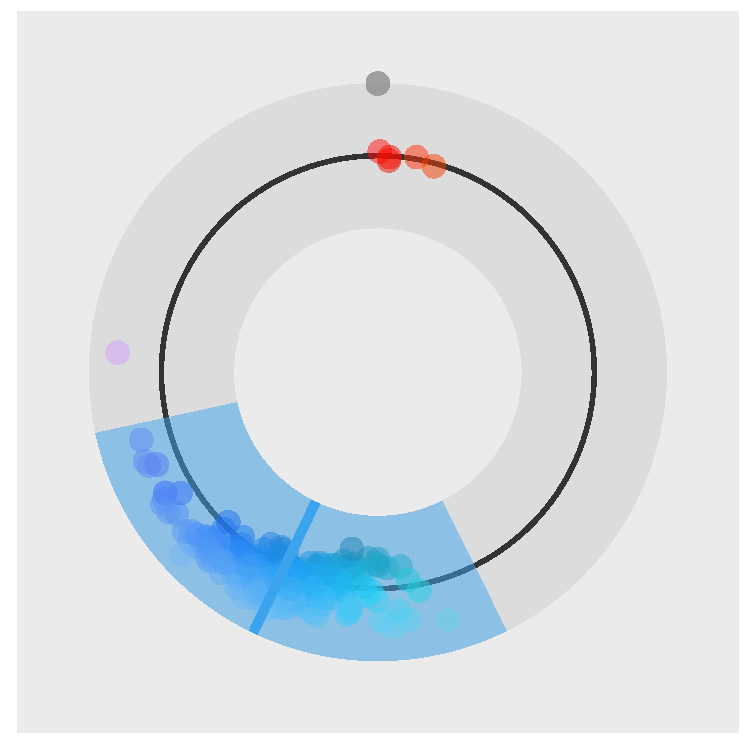
\includegraphics[width=\linewidth]{single_column.pdf}
%	\caption{\textbf{A random visualization.} This is an example of a figure that spans only across one of the two columns.}
%	\label{fig:column}
%\end{figure}

%On the other hand, \figurename~\ref{fig:whole} is an example of a figure that spans across the whole page (across both columns) of the report.
%
% \begin{figure*} makes the figure take up the entire width of the page
%\begin{figure*}[ht]\centering 
%	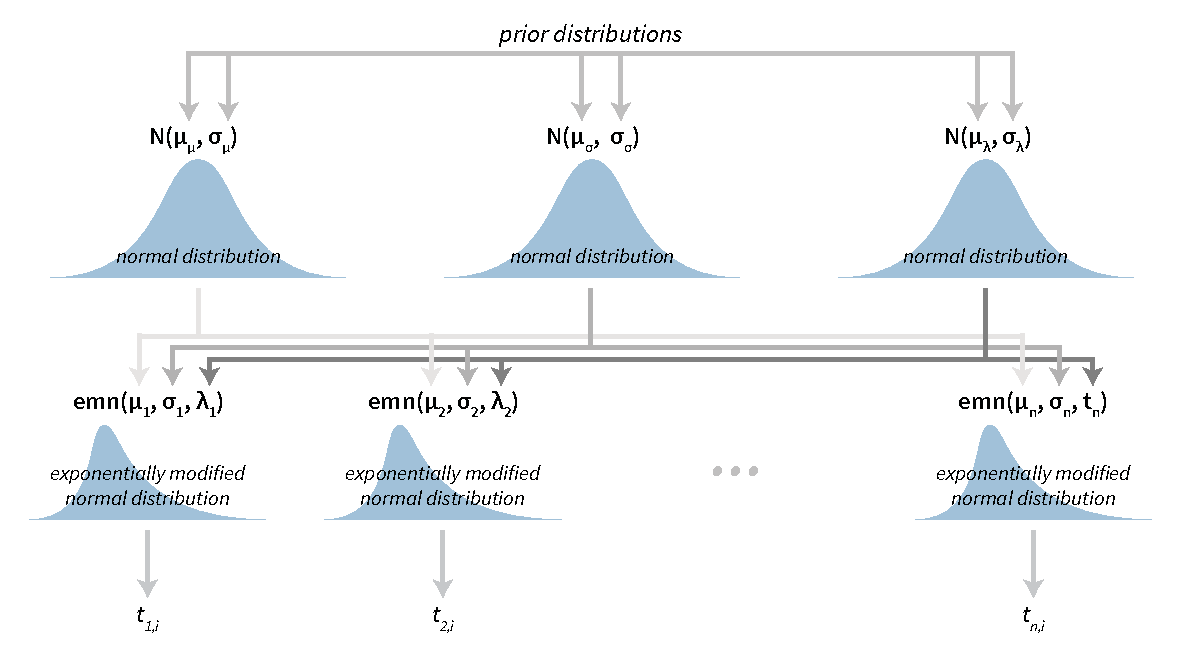
\includegraphics[width=\linewidth]{whole_page.pdf}
%	\caption{\textbf{Visualization of a Bayesian hierarchical model.} This is an example of a figure that spans the whole width of the report.}
%	\label{fig:whole}
%\end{figure*}


%\subsection*{Tables}

%Use the table environment to insert tables.

%\begin{table}[hbt]
%	\caption{Table of grades.}
%	\centering
%	\begin{tabular}{l l | r}
%		\toprule
%		\multicolumn{2}{c}{Name} \\
%		\cmidrule(r){1-2}
%		First name & Last Name & Grade \\
%		\midrule
%		John & Doe & $7.5$ \\
%		Jane & Doe & $10$ \\
%		Mike & Smith & $8$ \\
%		\bottomrule
%	\end{tabular}
%	\label{tab:label}
%\end{table}


%\subsection*{Code examples}

%You can also insert short code examples. You can specify them manually, or insert a whole file with code. Please avoid inserting long code snippets, advisors will have access to your repositories and can take a look at your code there. If necessary, you can use this technique to insert code (or pseudo code) of short algorithms that are crucial for the understanding of the manuscript.

%\lstset{language=Python}
%\lstset{caption={Insert code directly from a file.}}
%\lstset{label={lst:code_file}}
%\lstinputlisting[language=Python]{code/example.py}

%\lstset{language=R}
%\lstset{caption={Write the code you want to insert.}}
%\lstset{label={lst:code_direct}}
%\begin{lstlisting}
%import(dplyr)
%import(ggplot)

%ggplot(diamonds,
%	   aes(x=carat, y=price, color=cut)) +
%  geom_point() +
%  geom_smooth()
%\end{lstlisting}

%------------------------------------------------

\section*{Results}

\begin{table}[hbt]
	\caption{Table of baseline results using DistilBERT pre-trained on SQuAD before and after fine-tuning on our data.}
	\centering
    \label{tab:baseline_fine_tuning}
    \scalebox{0.75}{
    	\begin{tabular}{l | c c c c c c }
    		\toprule
    		& Bertscore & & & & SQuAD & \\
    		\cmidrule(r){2-4} \cmidrule(r){6-7}
    		Model & F1 & Precision & Recall & Bleu & Exact Match & F1 \\
            \midrule
    		Basline    & $87.5$ & $85.9$ & $89.4$ & $8.9$ & $35.7$ & $48.0$ \\
    		Fine-Tuned & $89.0$ & $87.5$ & $91.0$ & $9.2$ & $37.5$ & $49.1$ \\
    		\bottomrule
    	\end{tabular}
     }
\end{table}

Table~\ref{tab:baseline_fine_tuning} shows the effects of fine-tuning the DistilBERT model, that has already been pre-trained for the QA task.

%Use the results section to present the final results of your work. Present the results in a objective and scientific fashion. Use visualisations to convey your results in a clear and efficient manner. When comparing results between various techniques use appropriate statistical methodology.

%\subsection*{More random text}

%This text is inserted only to make this template look more like a proper report. Lorem ipsum dolor sit amet, consectetur adipiscing elit. Etiam blandit dictum facilisis. Lorem ipsum dolor sit amet, consectetur adipiscing elit. Interdum et malesuada fames ac ante ipsum primis in faucibus. Etiam convallis tellus velit, quis ornare ipsum aliquam id. Maecenas tempus mauris sit amet libero elementum eleifend. Nulla nunc orci, consectetur non consequat ac, consequat non nisl. Aenean vitae dui nec ex fringilla malesuada. Proin elit libero, faucibus eget neque quis, condimentum laoreet urna. Etiam at nunc quis felis pulvinar dignissim. Phasellus turpis turpis, vestibulum eget imperdiet in, molestie eget neque. Curabitur quis ante sed nunc varius dictum non quis nisl. Donec nec lobortis velit. Ut cursus, libero efficitur dictum imperdiet, odio mi fermentum dui, id vulputate metus velit sit amet risus. Nulla vel volutpat elit. Mauris ex erat, pulvinar ac accumsan sit amet, ultrices sit amet turpis.

%Phasellus in ligula nunc. Vivamus sem lorem, malesuada sed pretium quis, varius convallis lectus. Quisque in risus nec lectus lobortis gravida non a sem. Quisque et vestibulum sem, vel mollis dolor. Nullam ante ex, scelerisque ac efficitur vel, rhoncus quis lectus. Pellentesque scelerisque efficitur purus in faucibus. Maecenas vestibulum vulputate nisl sed vestibulum. Nullam varius turpis in hendrerit posuere.

%Nulla rhoncus tortor eget ipsum commodo lacinia sit amet eu urna. Cras maximus leo mauris, ac congue eros sollicitudin ac. Integer vel erat varius, scelerisque orci eu, tristique purus. Proin id leo quis ante pharetra suscipit et non magna. Morbi in volutpat erat. Vivamus sit amet libero eu lacus pulvinar pharetra sed at felis. Vivamus non nibh a orci viverra rhoncus sit amet ullamcorper sem. Ut nec tempor dui. Aliquam convallis vitae nisi ac volutpat. Nam accumsan, erat eget faucibus commodo, ligula dui cursus nisi, at laoreet odio augue id eros. Curabitur quis tellus eget nunc ornare auctor.


%------------------------------------------------

\section*{Discussion}
Thus far we have identified the main approaches for solving our problem and defined the pipeline we need to implement.
We started by fine tuning a model for the extractive approach and shown that fine tuning on our domain specific data improves the performance of the model.
When we receive the data written by the banking expert we plan on using that data to fine tune our models as it should be higher in quality.
Knowing that this approach should work we now plan on firstly adapting a context retriever to extract the relevant contexts from the yearly reports.
After this we plan to fine tune additional model(s) for the extractive approach and also try out the generative approach.
Finally we plan on identifying more evaluation protocols one of which would possibly be human evaluation where we would manually check the answers output by the models.

%Use the Discussion section to objectively evaluate your work, do not just put praise on everything you did, be critical and exposes flaws and weaknesses of your solution. You can also explain what you would do differently if you would be able to start again and what upgrades could be done on the project in the future.


%------------------------------------------------

\section*{Acknowledgments}

%Here you can thank other persons (advisors, colleagues ...) that contributed to the successful completion of your project.


%----------------------------------------------------------------------------------------
%	REFERENCE LIST
%----------------------------------------------------------------------------------------
\bibliographystyle{unsrt}
\bibliography{report}


\end{document}